\documentclass[aspectratio=169]{beamer}

\usepackage{graphicx}
\DeclareGraphicsExtensions{.pdf,.png,.jpg}
\graphicspath{{./fig/}}
\usetheme[russian]{vega}

\addbibresource{refs.bib}


\newcommand{\cA}{\mathcal{A}}
\newcommand{\cB}{\mathcal{B}}
\newcommand{\cC}{\mathcal{C}}
\newcommand{\cN}{\mathcal{N}}

\subtitle{ЛЕТНИЙ НАУЧНЫЙ ВЫЕЗД 2023}
\title{To sell or not to sell? That is the question.}
\author{Артемий Сазонов, Данил Лёгенький}
\institute{Механико-математический факультет МГУ имени М.В. Ломоносова}
\date{Июль 24, 2023}
\supervisor{Антон Филатов, Вадим Мещеряков}

\AtBeginSection{\begin{frame}\frametitle{\textTableofcontents}\tableofcontents[currentsection,hideallsubsections]\end{frame}}

\begin{document}
    \maketitle

    \section{Немного о задаче}
    
        \begin{frame}{Терминология}
        \begin{block}{Определение}
            Ордер -- это заявленное в определенное время подачи обязательство купить или продать определенный объем актива по цене не выше или, соответственно, не ниже заданной.
        \end{block}
            Ордеры, которые исполняются мгновенно по прибытии, называются \emph{рыночными} ордерами. Ордера, которые не совпадают по прибытии, называются \emph{лимитными} 
            (предельными) ордерами. Математически, ордер может быть описан вектором, состоящим из 4-х параметров: $x = (\epsilon_x, p_x, v_x, t_x) $, где 
            $\epsilon_x = \pm 1 $ ($\epsilon_x = + 1$ -- означает, что этот ордер -- ордер на покупку, и, соответственно, $\epsilon_x = - 1$ -- ордер 
            на продажу), $p_x$ -- цена, $v_x$ -- объем, $t_x$ -- время подачи ордера.
        \end{frame}
        
        \begin{frame}{Терминология}
            Книга лимитных ордеров (LOB) -- это  
            набор выявленных неудовлетворенных намерений купить или продать актив в определенный момент времени.

            Точнее, LOB $L(t)$ -- это набор всех лимитных ордеров для данного актива на данной платформе в момент времени $t$.   
            LOB можно представить в следующем виде
            \begin{equation*}
                L(t) = \mathcal{A}(t) \sqcup \mathcal{B}(t),
            \end{equation*}
            где $\mathcal{A}(t)$ - набор всех лимитных ордеров на продажу, $\mathcal{B}(t)$ - набор всех лимитных ордеров на покупку. 
        \end{frame}

        \begin{frame}{Терминология}
            \begin{itemize}
            
                \item Цена спроса (bid) в момент времени $t$ является самой высокой заявленной ценой среди лимитных ордеров на покупку в момент времени $t$: 
                \begin{equation*}
                    p_b(t) = \max\limits_{x \in \mathcal B(t)} p_x.
                \end{equation*}
        
                \item Цена предложения (ask) в момент времени $t$ является самой низкой заявленной ценой среди лимитных ордеров на продажу в момент времени $t$:
                \begin{equation*}
                    p_a(t) = \min\limits_{x \in \mathcal A(t)} p_x.
                \end{equation*}

                \item  Средняя цена (mid) и спред цены (spread) в момент времени $t$ равны
                \begin{equation*}
                    p_m(t) = \frac{p_a(t) + p_b(t)}{2}, \qquad s(t) = p_a(t) - p_b(t).
                \end{equation*}
                
            \end{itemize} 
        \end{frame}

        \begin{frame}{Терминология}
            Предположим, что у нас есть $W$ лотов некоторого актива, который мы хотим продать за время $T$. Разделим $T$ на $L$ интервалов длины $\tau = T/L$, и определим $t_k = k\tau, \; k = 0,1, \ldots, L$.
        
            \begin{block}{Определение}
                Торговая траектория - это процесс $(w_k)_{k = 0, \ldots, L}$, где $w_k$ - число лотов, которые мы продолжаем удерживать момент времени $t_k$. 
                Торговый список -- первая разность торговой траектории -- $(A_k)_{k \in \mathcal L}, \; \mathcal L = \{1,2,\ldots, L \}$, где $A_k$ - число лотов, которые мы продаем в момент времени $t_k$. 
                Торговая стратегия - это правило, по которому определяется $A_k$ в момент времени $t_k$ по имеющийся информации к этому моменту времени. 
            \end{block}
        \end{frame}

        \begin{frame}{Постановка задачи}
            Рассмотрим следующую ситуацию: мы хотим продать/купить какое-то количество некоторого актива, посылая последовательность рыночных ордеров.
            По закону спроса и предложения, текущая рыночная цена актива движется в направлении рыночного ордера.
            этот эффект называется \emph{влиянием на цену} (price impact). Но если мы держим позицию достаточно долго, то мы берем на себя значительный \emph{рыночный риск}.
            Эвристически проблема оптимального исполнения сделок записывается следующим образом:
            \begin{equation*}
                (\hat A_1, \dots, \hat A_L) = \operatorname*{arginf}_{A\in\mathbb{A}} \mathbb{L} (TC(A_1, \dots, A_L), \Phi(A_1, \dots, A_L)),
            \end{equation*}
            где $\mathbb{L}$ -- целевой функционал издержек и некоторой меры рыночного риска,
                $\mathbb{A}$ -- множество допустимых торговых списков.
        \end{frame}

    
    \section{Классические алгоритмы}
        \begin{frame}{Time-Weighted Average Price}
            Один из самых простых алгоритмов, которые можно придумать, это алгоритм, при котором $\forall i, j \in \mathcal L \ \ A_i \approx A_j$. 
            Вполне очевидно, что при отсутствии рыночного риска эта стратегия была бы оптимальной.
        \end{frame}

        \begin{frame}{Almgren-Chriss}{Описание модели}
            Пусть $\zeta_l, \; l \in \mathcal L$ - н.о.р. с нулевым средним и единичной дисперсией. Пусть также $g(A_l)$, $h(A_l)$ - функции постоянного и временного воздействия на цену соответственно. Тогда предполагается, что динамика бида задается как случайное блуждание:
            
            \begin{align*}
                &p_b(l) = p_b(l - 1) + \sigma \zeta_l - g(A_l), \\
                &\tilde p_b(l) = p_b(l - 1) - h(A_l),
            \end{align*}
            где $\tilde p_b(l)$ - эффективная цена, $\sigma > 0$.

        \end{frame}

        \begin{frame}{Almgren-Chriss}{Метрики}
            \begin{block}{Определение}
                Определим фиксацию траектории как общий номинальный торговый доход по завершении исполнения  
                \begin{equation*}
                    CP( A_{\cdot}, S_{\cdot}) = \sum_{l=1}^L A_{l}S_l,
                \end{equation*}
                где $S_{\cdot}$ - процесс цены актива. 
                Общие издержки торговой траектории определяется следующим образом:
                \begin{equation*}
                    \mathcal P = \mathcal P(W, A_{\cdot}, S_{\cdot}) = WS_0 - CP(A_{\cdot}, S_{\cdot}).
                \end{equation*}
            \end{block}
        \end{frame}

        \begin{frame}{Almgren-Chriss}{Постановка задачи}

                В случае AC модели, взяв в качестве процесса цены $S_l = p_b(l)$, получаем, что общие издержки торговой траектории выглядит следующим образом:
        
            \begin{equation*}
                \mathcal P = Wp_b(l) - \sum\limits_{l=1}^L \tilde p_b(l)A_l = \sum\limits_{l=1}^L ( g(A_l)w_l + h(A_l)A_l) - \sum\limits_{l=1}^L \sigma \zeta_l w_l .
            \end{equation*}

            Цель AC алгоритма состоит в решении следующей оптимизационной задачи 

            \begin{equation*}
                \E [ \mathcal P] + \lambda \var[\mathcal P] \to \min, \quad \lambda > 0.
            \end{equation*}

            Параметр $\lambda > 0$ интерепретируется как степень неприятия риска.

        \end{frame}

        \begin{frame}{Almgren-Chriss}{Решение задачи}

            В случае когда $g(x) = \gamma x, \; h(x) = \eta x $, поставленная оптимизационная задача решается явно и ее решение имеет следующий вид:

            \begin{align} 
                &A_l^{*} = \frac{2 \sinh(\kappa/2)}{\sinh(\kappa L)}\cosh(\kappa (L - l + 0.5) )W, \label{Al}\\
                &\kappa = \cosh^{-1}(0.5\tilde \kappa^2 + 1), \; \tilde \kappa = \frac{\lambda \sigma}{\eta - 0.5 \gamma}. \label{kappa}
            \end{align}

        \end{frame}


    \section{Online Machine Learning}

        \begin{frame}{Пару слов об OML и RL}
            \begin{figure}
                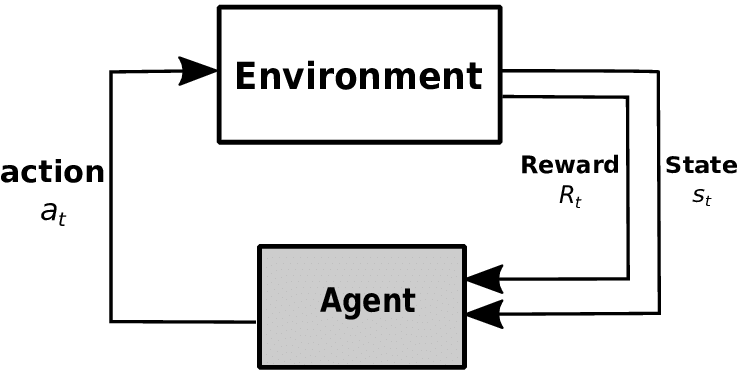
\includegraphics[width=0.8\textwidth]{Reinforcement-Learning-Agent-and-Environment}
            \end{figure}
        \end{frame}

        \begin{frame}{Пару слов об OML и RL}
            Мощным инструментом, который тесно связан с OML, и который используется для решения задач оптимального исполнения, являются марковские процессы принятия решений (MDP). MDP обеспечивают математическую основу для моделирования процесса принятия решений в стохастических средах, где результаты действий неопределены.
            Формально, MDP определяется набором $(\mathcal S, \mathcal A, P, R)$, где
        
            \begin{itemize}
        
                \item $\mathcal S$ - представляет собой набор состояний окружающей среды,
                
                \item $\mathcal A$ - представляет собой набор действий, которые могут быть предприняты агентом,
        
                \item $P$ - функция переходов, которая определяет вероятность перехода из одного состояния в другое,
        
                \item $R$ - функция вознаграждения. которая количественно определяет желательность или полезность пребывания в определенном состоянии или совершения определенного действия.
            \end{itemize}
        
        \end{frame}

        \begin{frame}{GLOBE}{Пререквизиты}

            Предположим, что мы хотим продать $W_1, W_2, \ldots, W_N$ лотов некоторого актива, за периоды времени $[0, T], [T, 2T], \ldots, [(N-1)T, NT]$ соотвественно. Такие пероды времени будем называть раундами.
            Как и раньше, каждый раунд делится еще на $L$ равных интервалов длины $\tau = T/L$, и аналогично тому, что было раньше, на каждом раунде $\rho$ определяются $(A_l^\rho)_{l \in \mathcal L}, \; (w_l^\rho)_{l \in \mathcal L \cup \{0\}}$.

        \end{frame}

        \begin{frame}{GLOBE}{Пререквизиты}

            Введем следующие множества:
        
            \begin{itemize}
                \item $\mathcal M , \; |\mathcal M| < \infty$ - множество состояний рынка, которое будет использоваться для определения динамики бида, как марковского процесса с конечным числом состояний:
                \begin{equation*}
                    \mathcal M \ni M_l^\rho = \frac {p_b(\rho, l) - p_b(\rho, 1)}{\sigma_\rho}.
                \end{equation*}
                
                \item $\mathcal I = \{0,1, 2, \ldots, W_{\max} \}$ - множество частных состояний или множество возможных значений $w_l^\rho$. Более того, предположим, что $W_\rho \in [W_{\min}, W_{\max}], \; 0<W_{\min} \leqslant W_{\max}, \; \rho \in \{1, 2, \ldots, N \}$. Частное состояние в слоте $l$ в раунде $\rho$ обозначим через $I_l^\rho \in \mathcal I$. Считаем, что $I_1^\rho = W_\rho$.
            \end{itemize}
        
        \end{frame}

        \begin{frame}{GLOBE}{Пререквизиты}
            В качестве $\sigma_\rho$ берется
            \begin{align*}
                &\sigma_\rho = \sqrt{\frac {\sum\limits_{j=1}^{\rho -1}[Ret(j) - \mu_\rho ]^2} {\rho - 1} },\\
                &\mu_\rho =  \frac1{\rho -1}\sum_{j=1}^{\rho -1} Ret(j) , \quad Ret(j) =  \log(p_m(\rho, L)/p_m(\rho, 1) ).
            \end{align*}
            Вводится множество действий на каждом слоте каждого раунда $\mathcal A_l^\rho = \{0,1,2,\ldots, A_l^\rho \}$, где $A_l^\rho = A_l^{*}$, которые находятся из уравнений \eqref{Al} - \eqref{kappa} в начале каждого раунда. 
        \end{frame}

        \begin{frame}{GLOBE}{Пререквизиты}
            \begin{block}{Определение}
            Введем ошибку реализации:
                \begin{equation*}
                    IS_\rho = 1 - \sum\limits_{l = 1}^{L} \frac{A_l^\rho p_b(\rho, l)}{Wp_m(\rho , 1)}.
                \end{equation*}
                Тогда средние издержки за раунд определяются как
                \begin{equation*}
                    ACPR_\rho = \frac{1}{\rho} \sum\limits_{j=1}^\rho IS_j.
                \end{equation*}
            \end{block}

        \end{frame}

        \begin{frame}{GLOBE}{Пререквизиты}

            Заметим, что используя введенные выше обозначения, ошибка реализации переписывается в виде
            
            \begin{equation*}
                IS_\rho = \sum\limits_{l=1}^L C_{X_\rho}(M_l^\rho, A_l^\rho), \quad C_{X_\rho}(M_l^\rho, A_l^\rho) = \frac{1}{W_\rho p_m(\rho, 1)} \left[ A_l^\rho \left(\frac{B_1^\rho}{2} - M_l^\rho \sigma_\rho \right) \right],
            \end{equation*}
            
            где $B_l^\rho = p_a(\rho, l) - p_b(\rho, l), \; X_\rho = (W_\rho, p_m(\rho, 1), \sigma_\rho, B_1^\rho )$ - определяются в начале раунда, и не меняются в течение него. Обозначим множество возможных значений $X_\rho$ через $\mathcal X$.
        
        \end{frame}

        \begin{frame}{GLOBE}{Постановка задачи}
        
            На каждом раунде $\rho$ нахождение такой политики $\pi = (\pi_1, \pi_2, \ldots, \pi_L)$,
            \begin{equation*}
                \pi_l \colon \mathcal M \times \mathcal I \to \mathcal A_l^\rho ,
            \end{equation*}

            что она минимизирует
            \begin{equation*}
                \E \left[ C_{X_\rho}^\pi \right] = \E \left[ \sum\limits_{l=1}^L C_{X_\rho}(M_l^\rho, \pi_l (M_l^\rho, I_l^\rho) ) \right].
            \end{equation*}

            Данная задача решаетя в случае, если известна переходная функция $P$. Используя принцип оптимальности Беллмана, получаем, что решение данной оптимизационной задачи есть
            
            
        \end{frame}
        
        
        \begin{frame}{GLOBE}{Постановка задачи}

            \begin{align*}
                &V_l(M, I) =\min\limits_{a \in \mathcal A_l^\rho}\left[ Q(M, I, a) \right] =\min\limits_{a \in \mathcal A_l^\rho} \left[C_X(M, a) + \sum\limits_{M^\prime \in \mathcal M} P(M, M^\prime) V_{l+1}(M^\prime, I - a ) \right], \\
                &\pi_l(M,I) = \arg\min\limits_{a \in \mathcal A_l^\rho}Q(M, I, a), \quad V_L(M,I) = C_X(M,I), \; \pi_L(M,I) = I
            \end{align*}
            для любых $M \in \mathcal M, \; I \in \mathcal I, \; l \in \mathcal L \backslash \{L\}, \; X \in \mathcal X $.
            На практике данная задача решается методом динамического программирования. 
            Неизвестная функция $P(M, M^\prime)$ заменяется на эмпирический аналог $\hat P(M, M^\prime)$.

        \end{frame}

        \begin{frame}{GLOBE}{Постановка задачи}
            $\hat P(M, M^\prime)$ в начале каждого раунда обновляется следующим образом:
            \begin{align*}
                &N_\rho(M, M^\prime) = \sum\limits_{\rho^\prime = 1}^{\rho - 1} \sum\limits_{l = 1}^{L - 1} \mathbb I (M_{\rho^\prime}^l = M)\mathbb I (M_{\rho^\prime}^{l + 1} = M^\prime), \quad M, M^\prime \in \mathcal M, \\
                &N_\rho(M) = \sum\limits_{M^\prime \in \mathcal M} N_\rho(M, M^\prime), \quad M \in \mathcal M,\\
                &\hat P(M, M^\prime) = \frac{N_\rho(M, M^\prime) + \mathbb I (N_\rho(M) = 0 ) } {N_\rho (M) + |\mathcal M| \mathbb I (N_\rho(M) = 0 )} \quad M, M^\prime \in \mathcal M.
            \end{align*}
            $N_\rho(M, M^\prime), N_\rho(M)$ обновляются в конце каждого раунда.
            Оказывается, что если $W_{\max}$ достаточно мал, то $\mathcal A_l^\rho$ можно заменить на $\mathcal A_l^{*,\rho} = \{0, A_l^\rho \}$.
            
        \end{frame}

        \begin{frame}{GLOBE+}{Описание алгоритма}
            Был рассмотрен еще один алгоритм. Всё аналогично обычному алгоритму, который был описан выше, за исключением того, что $\mathcal A_l^\rho$ меняется на $\{0,1,\ldots 2A_l^\rho\}$.
            Само собой, теоретический результат с прошлого слайда в этом случае не применим.

        \end{frame}


    \section{Практическая реализация}

        \begin{frame}{Метрики}
            Все алгоритмы будут сравниваться по метрике $ACPR$ и связанной с ней $RI$.

            \begin{block}{Определение (Relative Improvement)}

                $RI$ показывает относительное снижение торговых
                издержек по сравнению с базовой моделью (TWAP, в нашем случае):
        
                \begin{equation*}
                    RI_\rho(alg) = \frac{ACPR_\rho(baseline) - ACPR_{\rho}(alg)  }{|ACPR_\rho(baseline)|}.
                \end{equation*}
                
            \end{block}
            
        \end{frame}
        
        \begin{frame}{TWAP}
        
            Отметим, что объем и ценовые уровни целочисленные. Поэтому имеет смысл все $A^\rho_l$ моделировать целочисленными, т.е. $A^\rho_l = [W_\rho/L], \; l \in \mathcal L \backslash \{L\} , \; A^\rho_L = [W_\rho/L] + (W_\rho - L[W_\rho/L])$, где $[x]$ - целая часть $x$. 

            Никаких дополнительных параметров не вводится, кроме числа раундов, для сравнения этого алгоритма с AC/GLOBE.
            
        \end{frame}

        \begin{frame}{AC}

            Аналогично предыдущему, $A^\rho_l = [A_l^{*, \rho}], \; l \in \mathcal L \backslash \{L\} , \; A^\rho_L = W_\rho - \sum\limits_{l=1}^{L-1}A_l^\rho$. В качестве дополнительных параметров на вход должны подаваться $\eta, \gamma$, а также число раундов, и число раундов для оценки $\sigma_\rho$ (напомним, что $\sigma_\rho$ можно определить лишь в начале второго раунда, и то в этом случае, она будет равна 0). 

        \end{frame}

        \begin{frame}{GLOBE и GLOBE+}
            В качестве $\mathcal A_l^{*, \rho}$ берется множество $\{0, [A_l^{*,\rho}]\}$ (для GLOBE+ множество действий: $\{0, 1, 2, \ldots, 2 [A_l^{*,\rho}] \} )$. Помимо параметров, которые передается в AC, передается также множество $\mathcal M$ которое оценивается по историческим данным. Во время оценки $\sigma_\rho$, множество $\mathcal M$ также будет обновляться. 
            Состояние рынка в слоте $l$ в раунде $\rho$ определяется как 
            \begin{equation*}
                M_l^\rho = \left[\frac {p_b(\rho, l) - p_b(\rho, 1)}{K\sigma_\rho} \right],
            \end{equation*}
            где $K \in \mathbb N$ передается в качестве дополнительного параметра, и нужен для того, чтобы уменьшить множество $\mathcal M$, мощность которого существенно влияет на сложность алгоритма.

        \end{frame}


    \section{Результаты}

        \begin{frame}{Параметры}
            \begin{itemize}
                \item Во всех тестах, если не оговорено иное, параметры брались одни и те же: $T = 50, W_\rho = 500, \; \gamma = 0, \; \eta = 0.002, \; \lambda = 0.02, \; N = 10, \; rounds\_for\_est = 15, \; K = 100\_000$. 

                \item При таком выборе $K$ число состояний в $\mathcal M$ порядка 10-20. Для алгоритма TWAP первые 15 раундов пропускались. 
            \end{itemize}  
        \end{frame}
        
        \begin{frame}{Бектест}
        
            \begin{figure}  
                \centering
                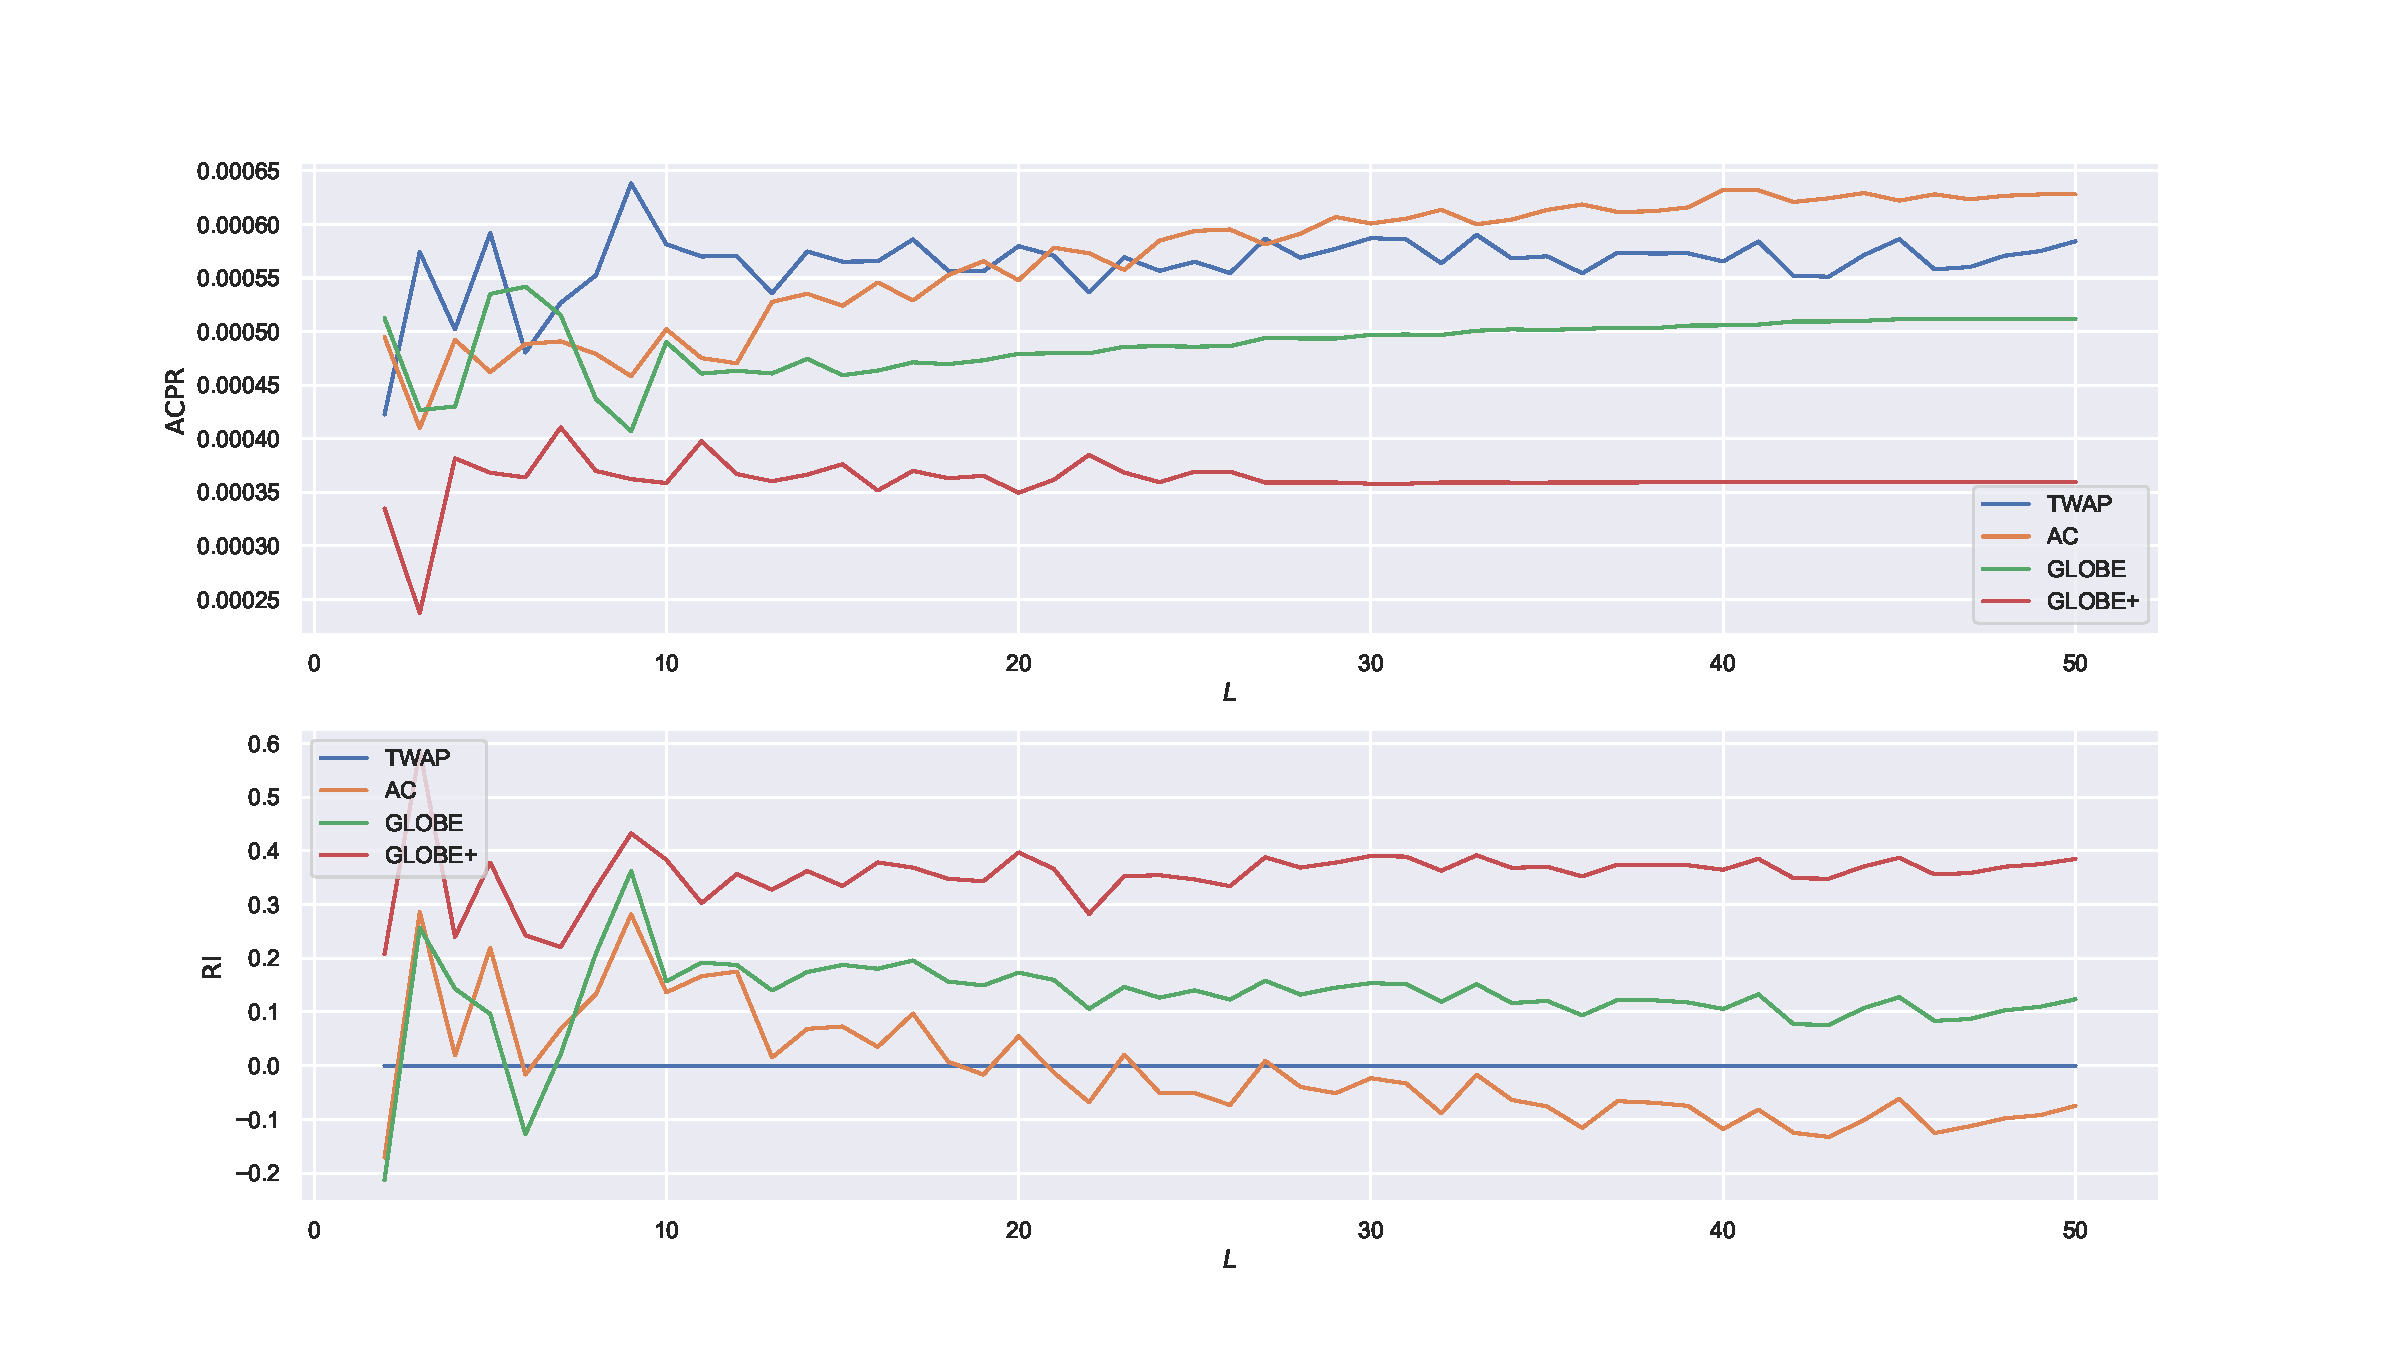
\includegraphics[width=0.83\linewidth]{USD_CNH_T+1 2022-10-04 T = 50 W = 500}
                \caption{USD\_CNH\_TOM 2022-10-04. $T = 50, W = 500$}
            \end{figure}

        \end{frame}

        \begin{frame}{Бектест}
        
            \begin{figure}  
                \centering
                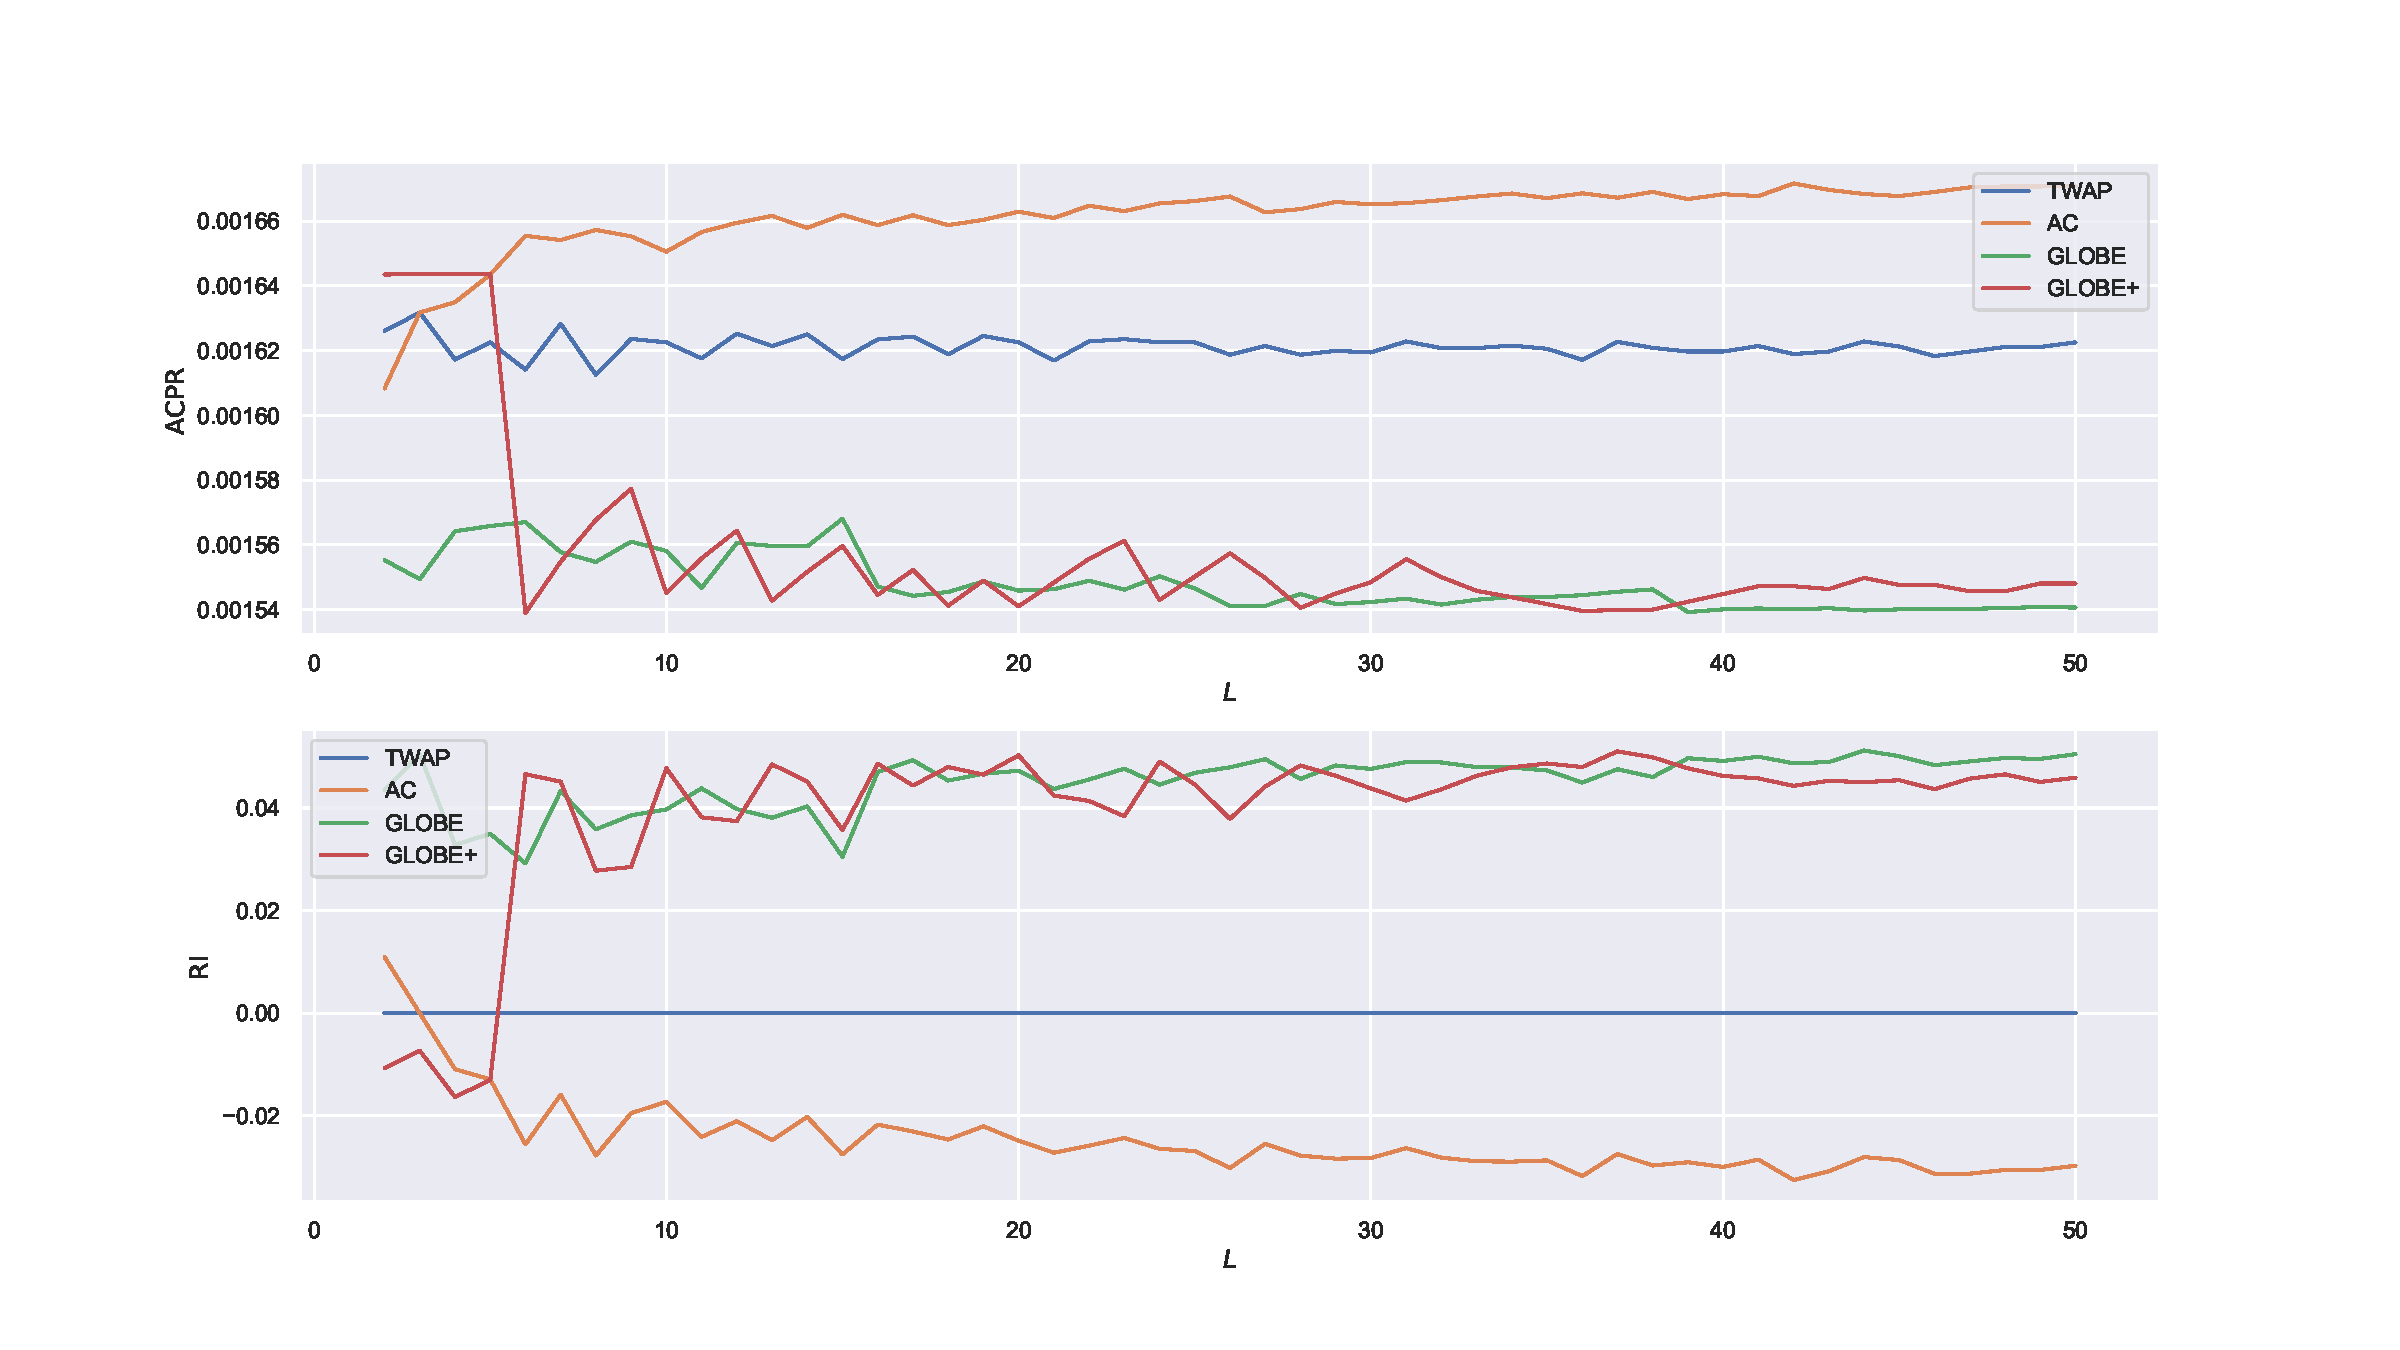
\includegraphics[width=0.83\linewidth]{USD_CNH_T+1 2022-11-15 T = 50 W = 500}
                \caption{USD\_CNH\_TOM 2022-11-15. $T = 50, W = 500$}
            \end{figure}

        \end{frame}

        \begin{frame}{Бектест}
        
            \begin{figure}  
                \centering
                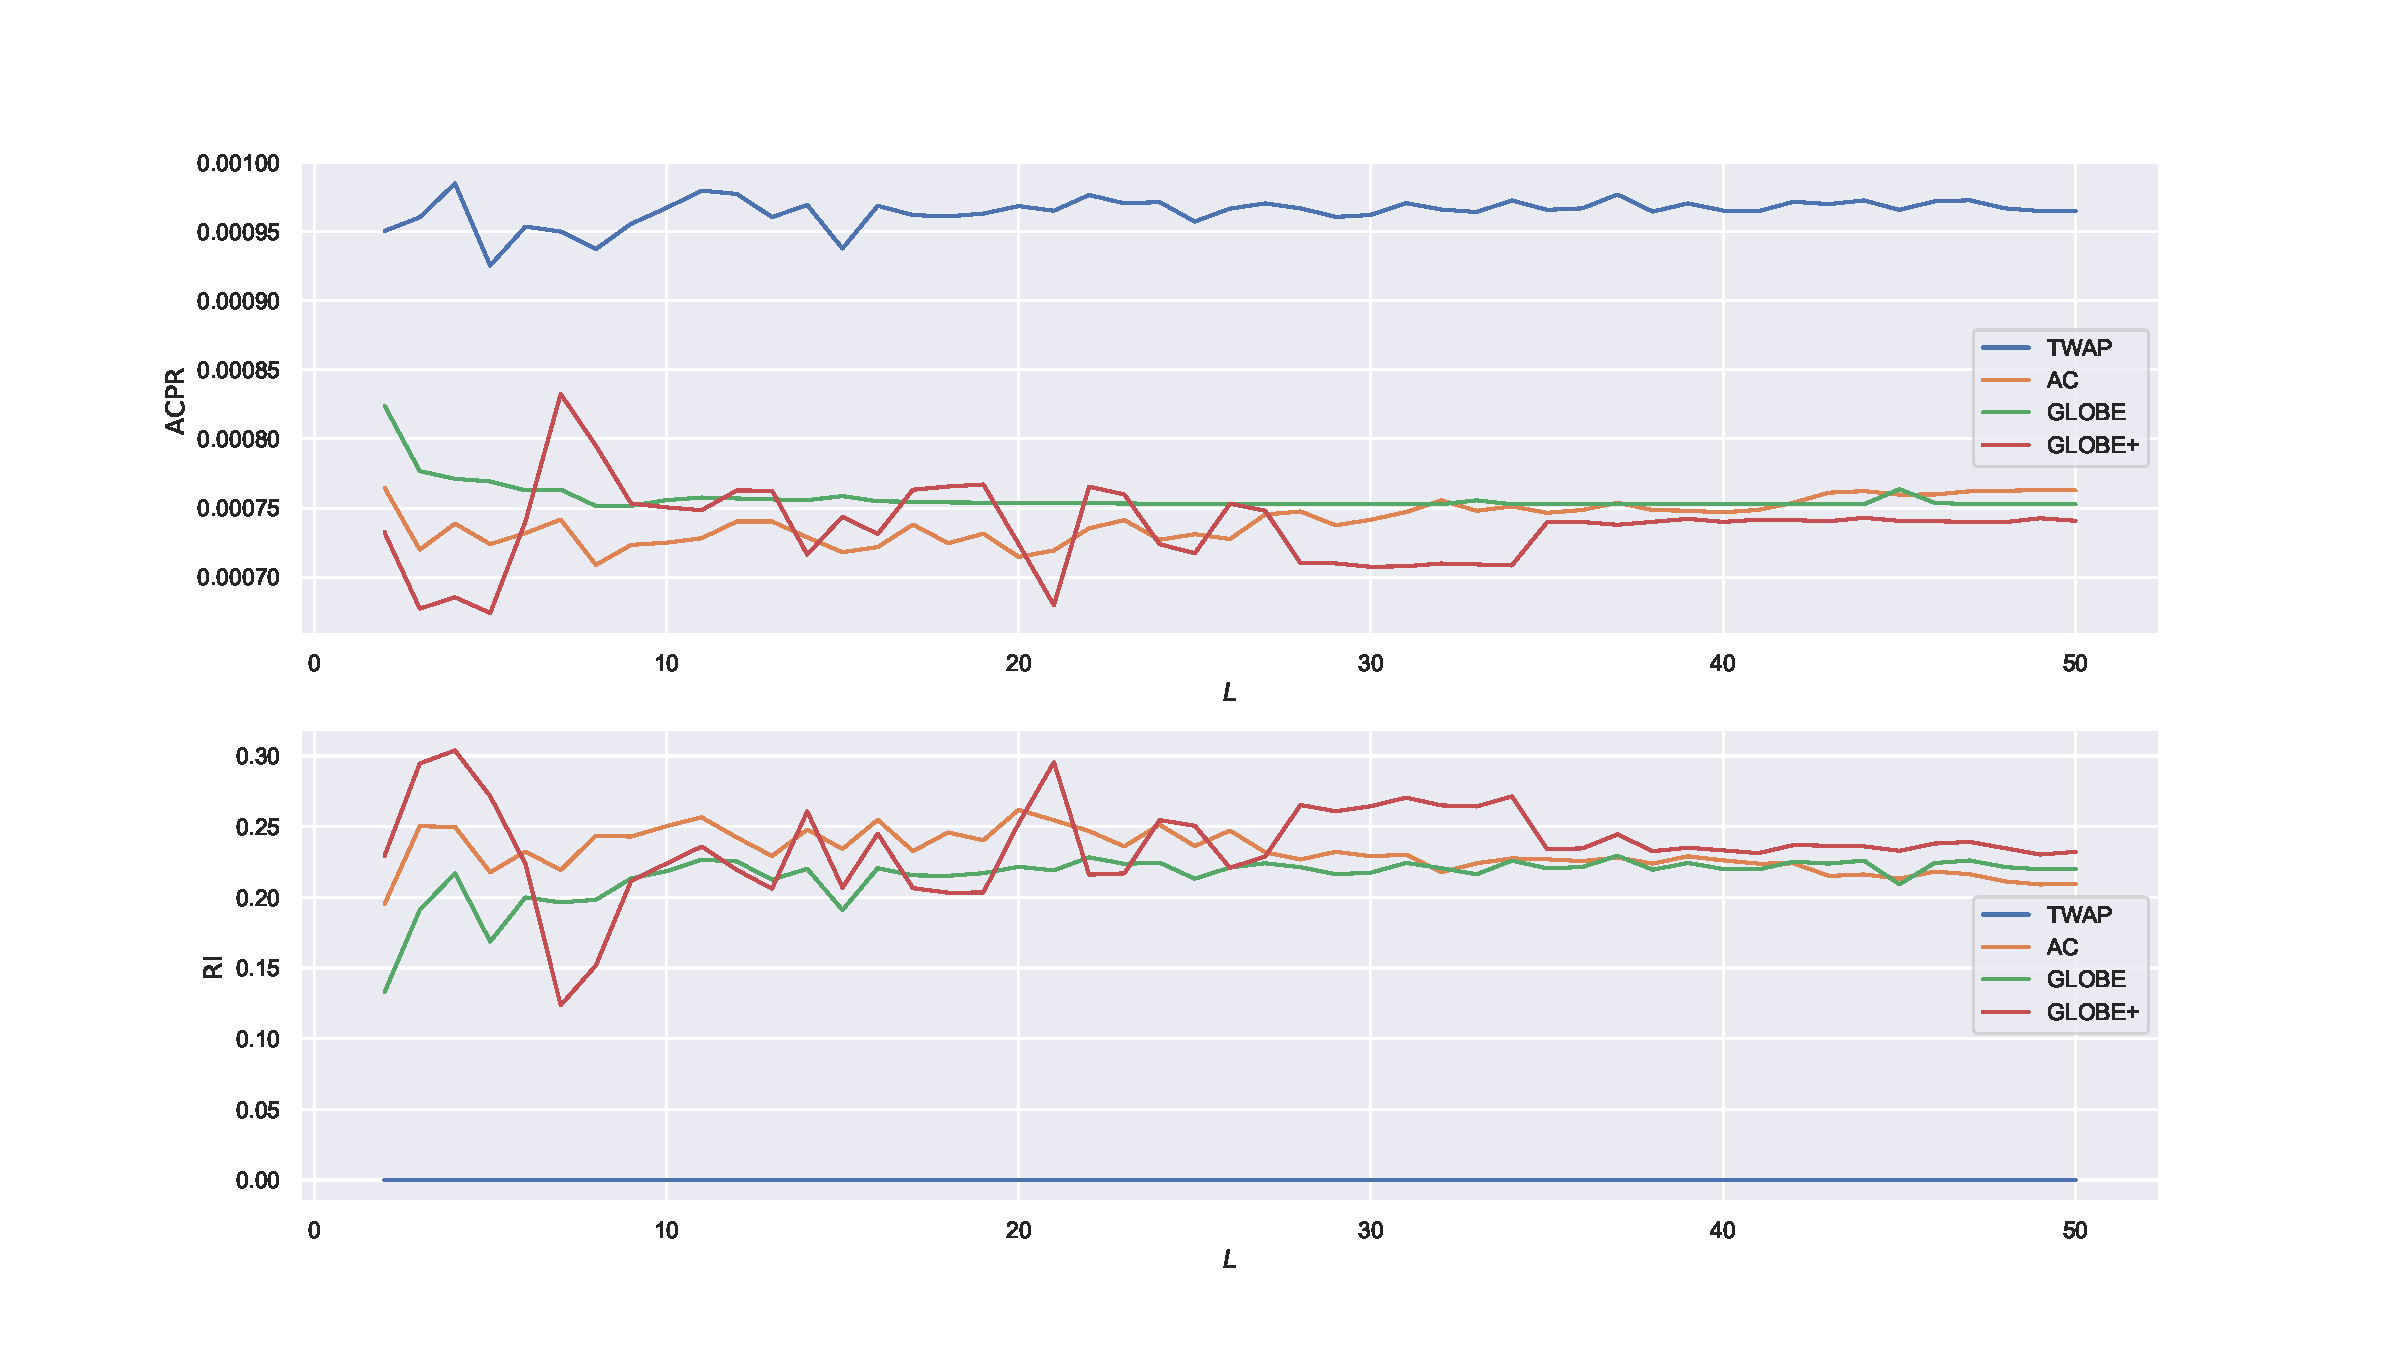
\includegraphics[width=0.83\linewidth]{USD_RUB_T+1 2022-10-20 T = 50 W = 500}
                \caption{USD\_RUB\_TOM 2022-11-15. $T = 50, W = 500$}
            \end{figure}

        \end{frame}

        \begin{frame}{Бектест}
        
            \begin{figure}  
                \centering
                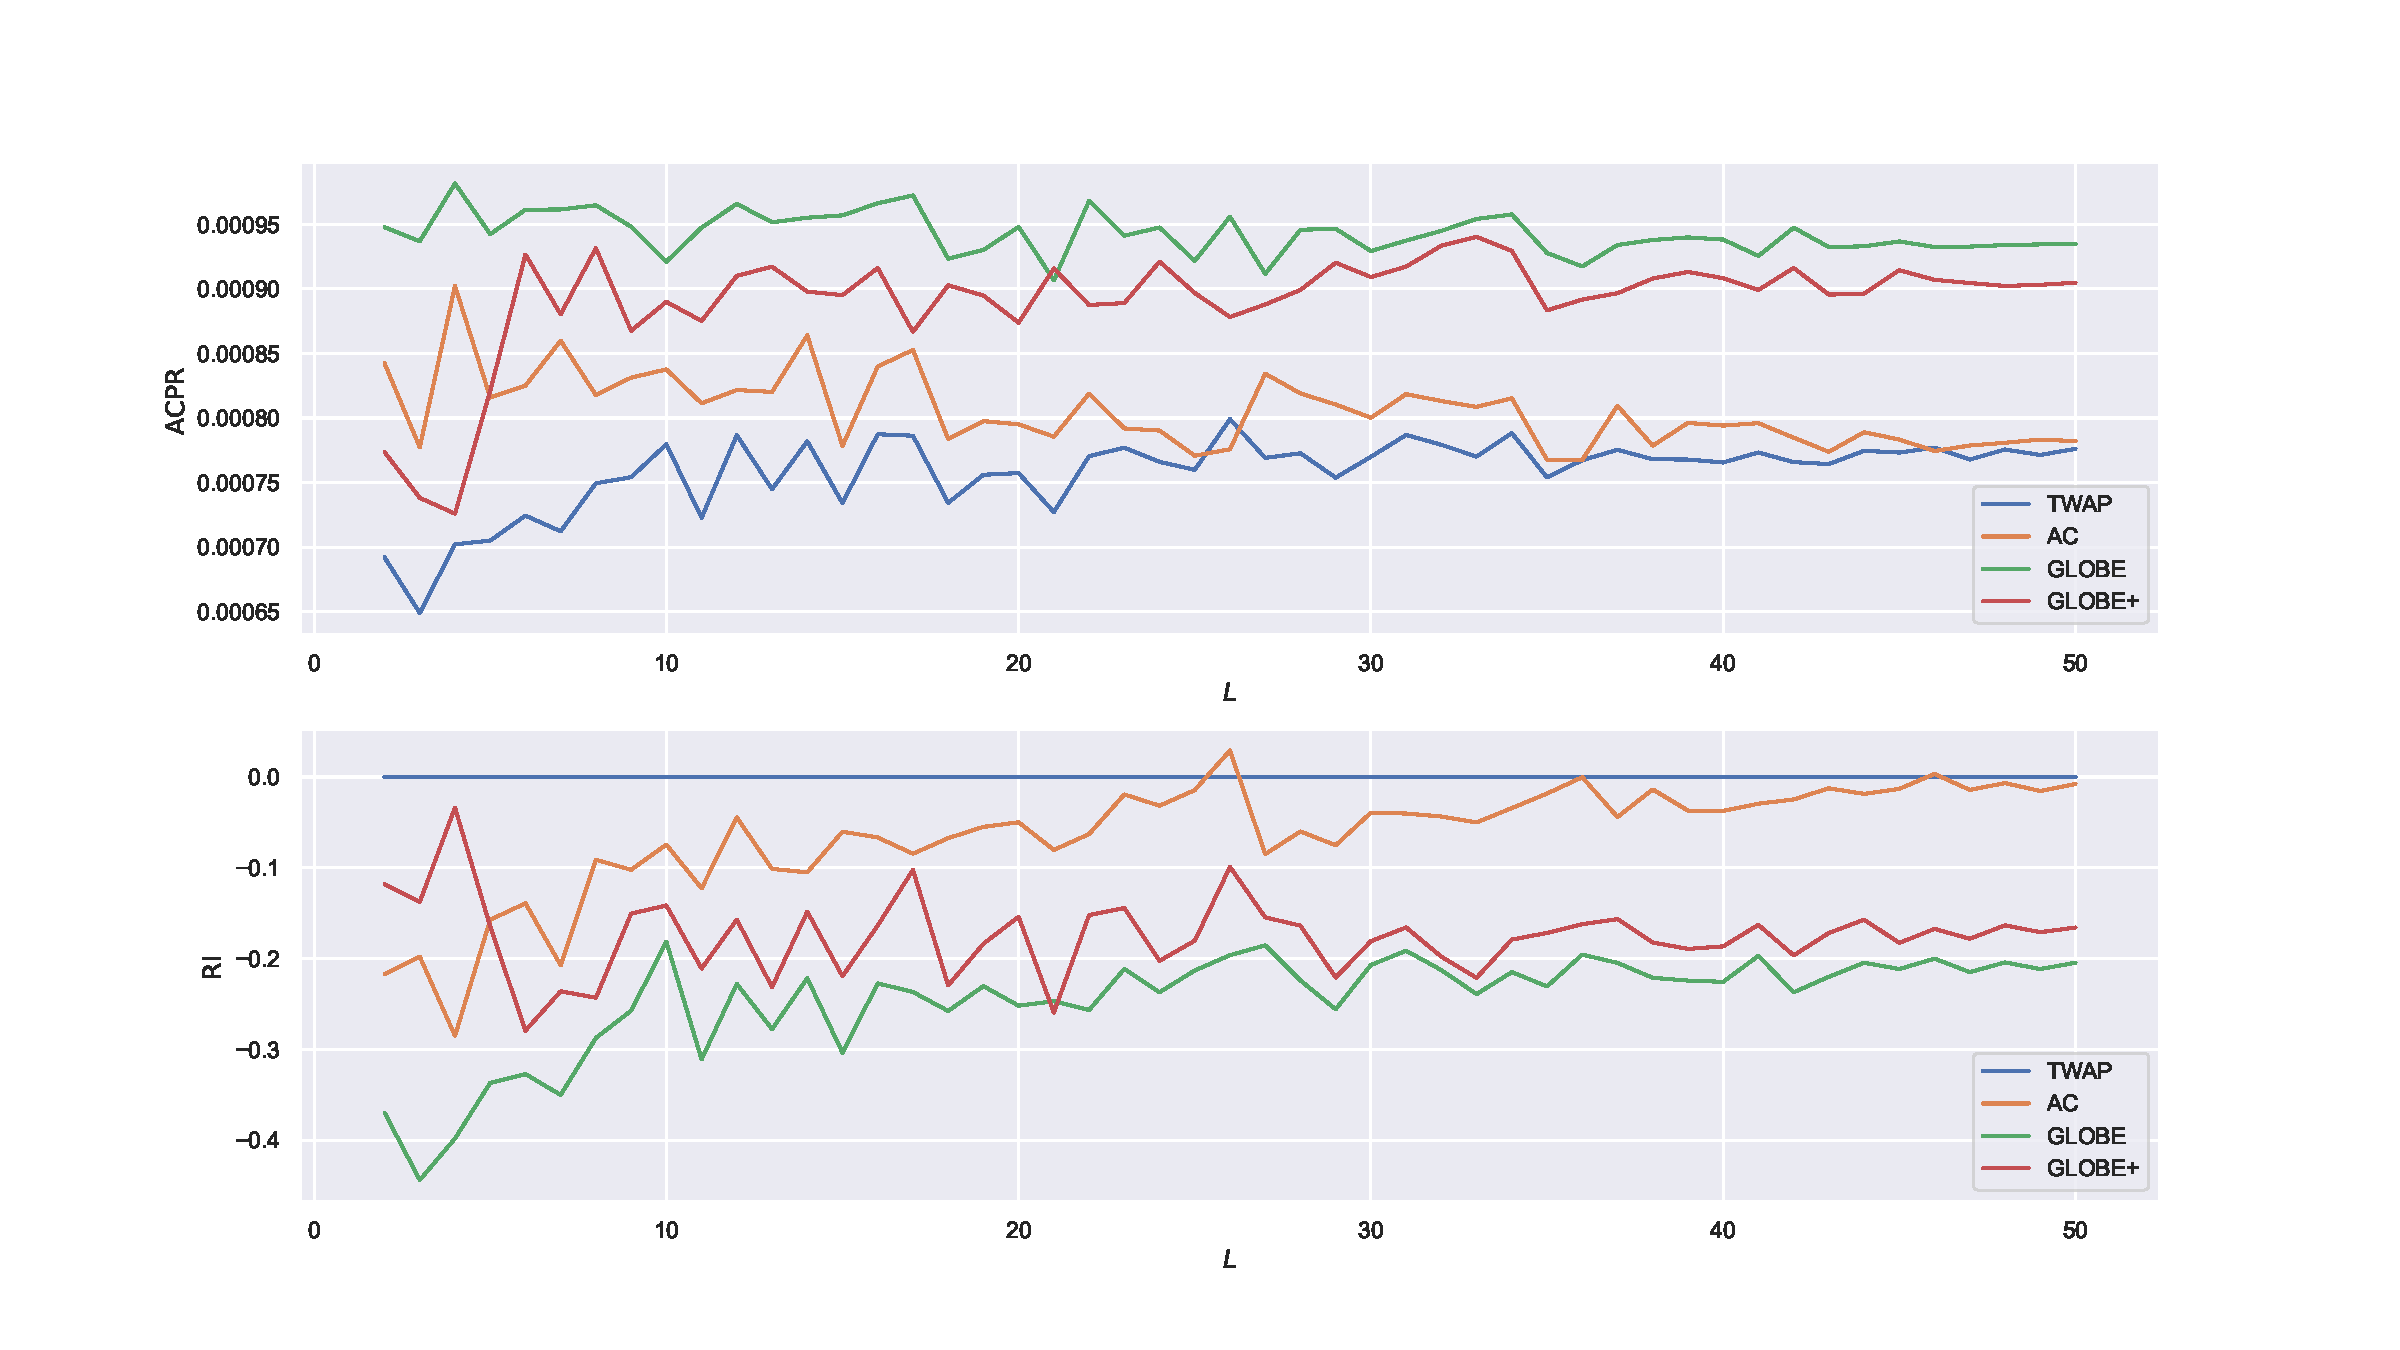
\includegraphics[width=0.83\linewidth]{USD_RUB_T+1 2022-10-28 T = 50 W = 500}
                \caption{USD\_RUB\_TOM 2022-10-28. $T = 50, W = 500$}
            \end{figure}

        \end{frame}


        \begin{frame}{Бектест -- Область неприменимости алгоритмов}
            %А теперь немного о том, что происходит, если брать объем сильно больше объема на уровне лучшего бида:  $W = 500\_000$ (сбивает 4 ценовых уровня).
            \begin{figure}  
                \centering
                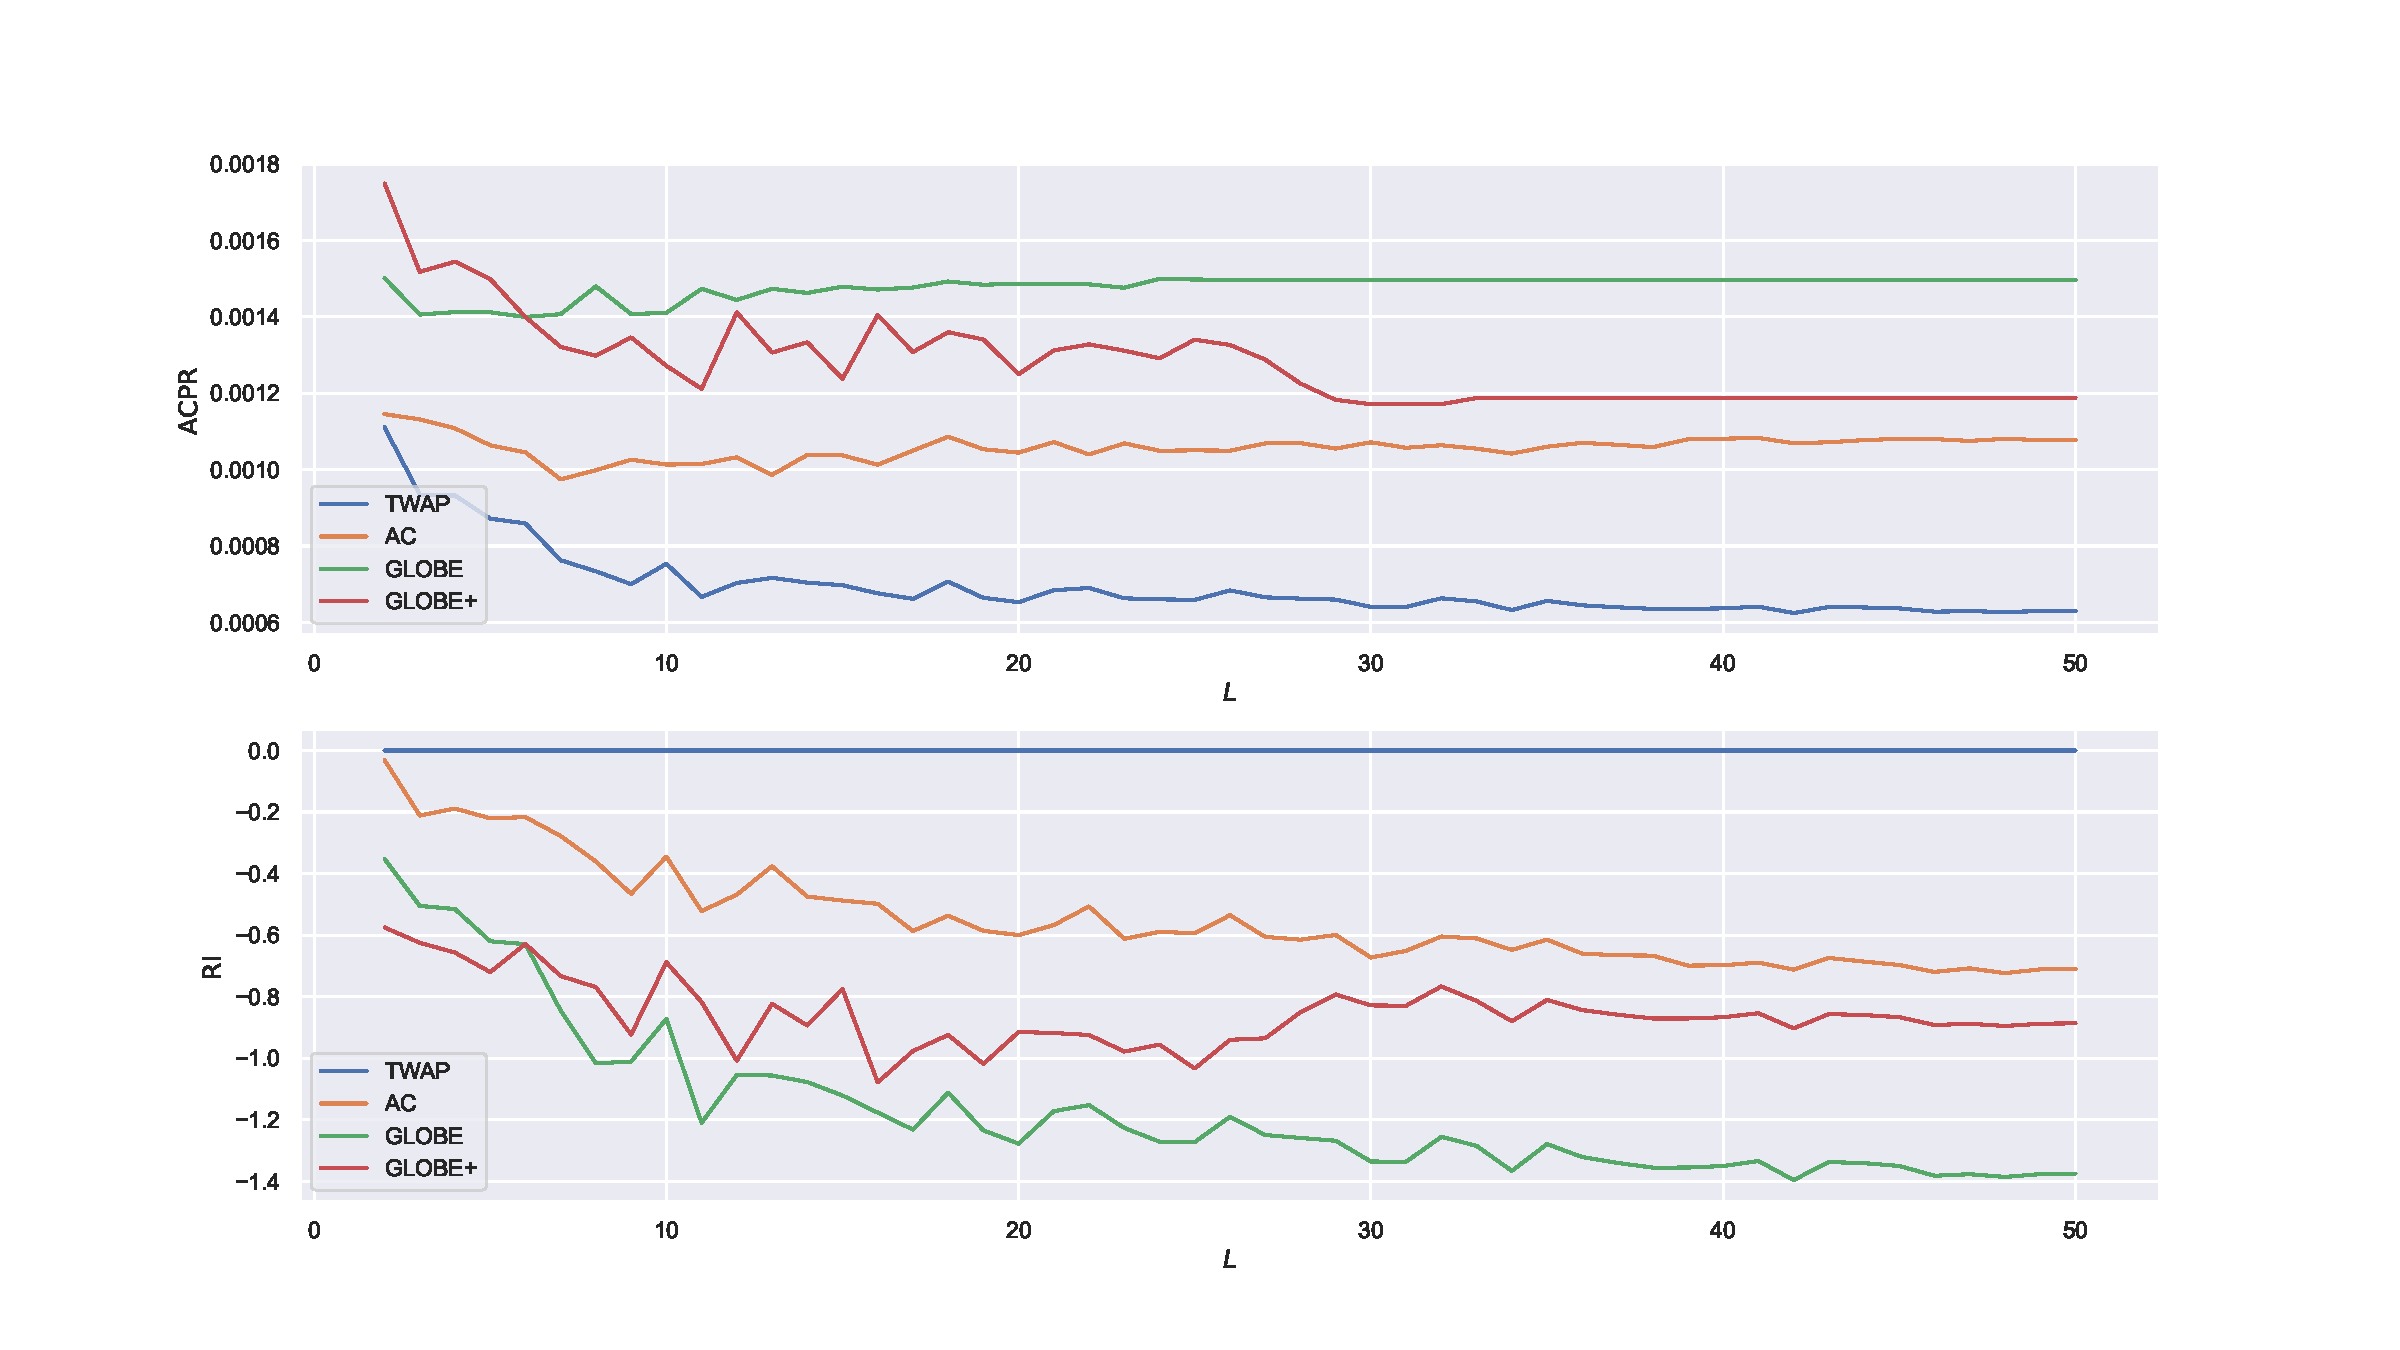
\includegraphics[width=0.83\linewidth]{USD_RUB_T+1 2022-10-04 T = 50 W = 500, x10000}
                \caption{USD\_RUB\_TOM 2022-10-04. $T = 50, W = 500\_000$}
            \end{figure}
            
        \end{frame}

        \begin{frame}{Бектест -- Область неприменимости алгоритмов}

            \begin{figure}  
                \centering
                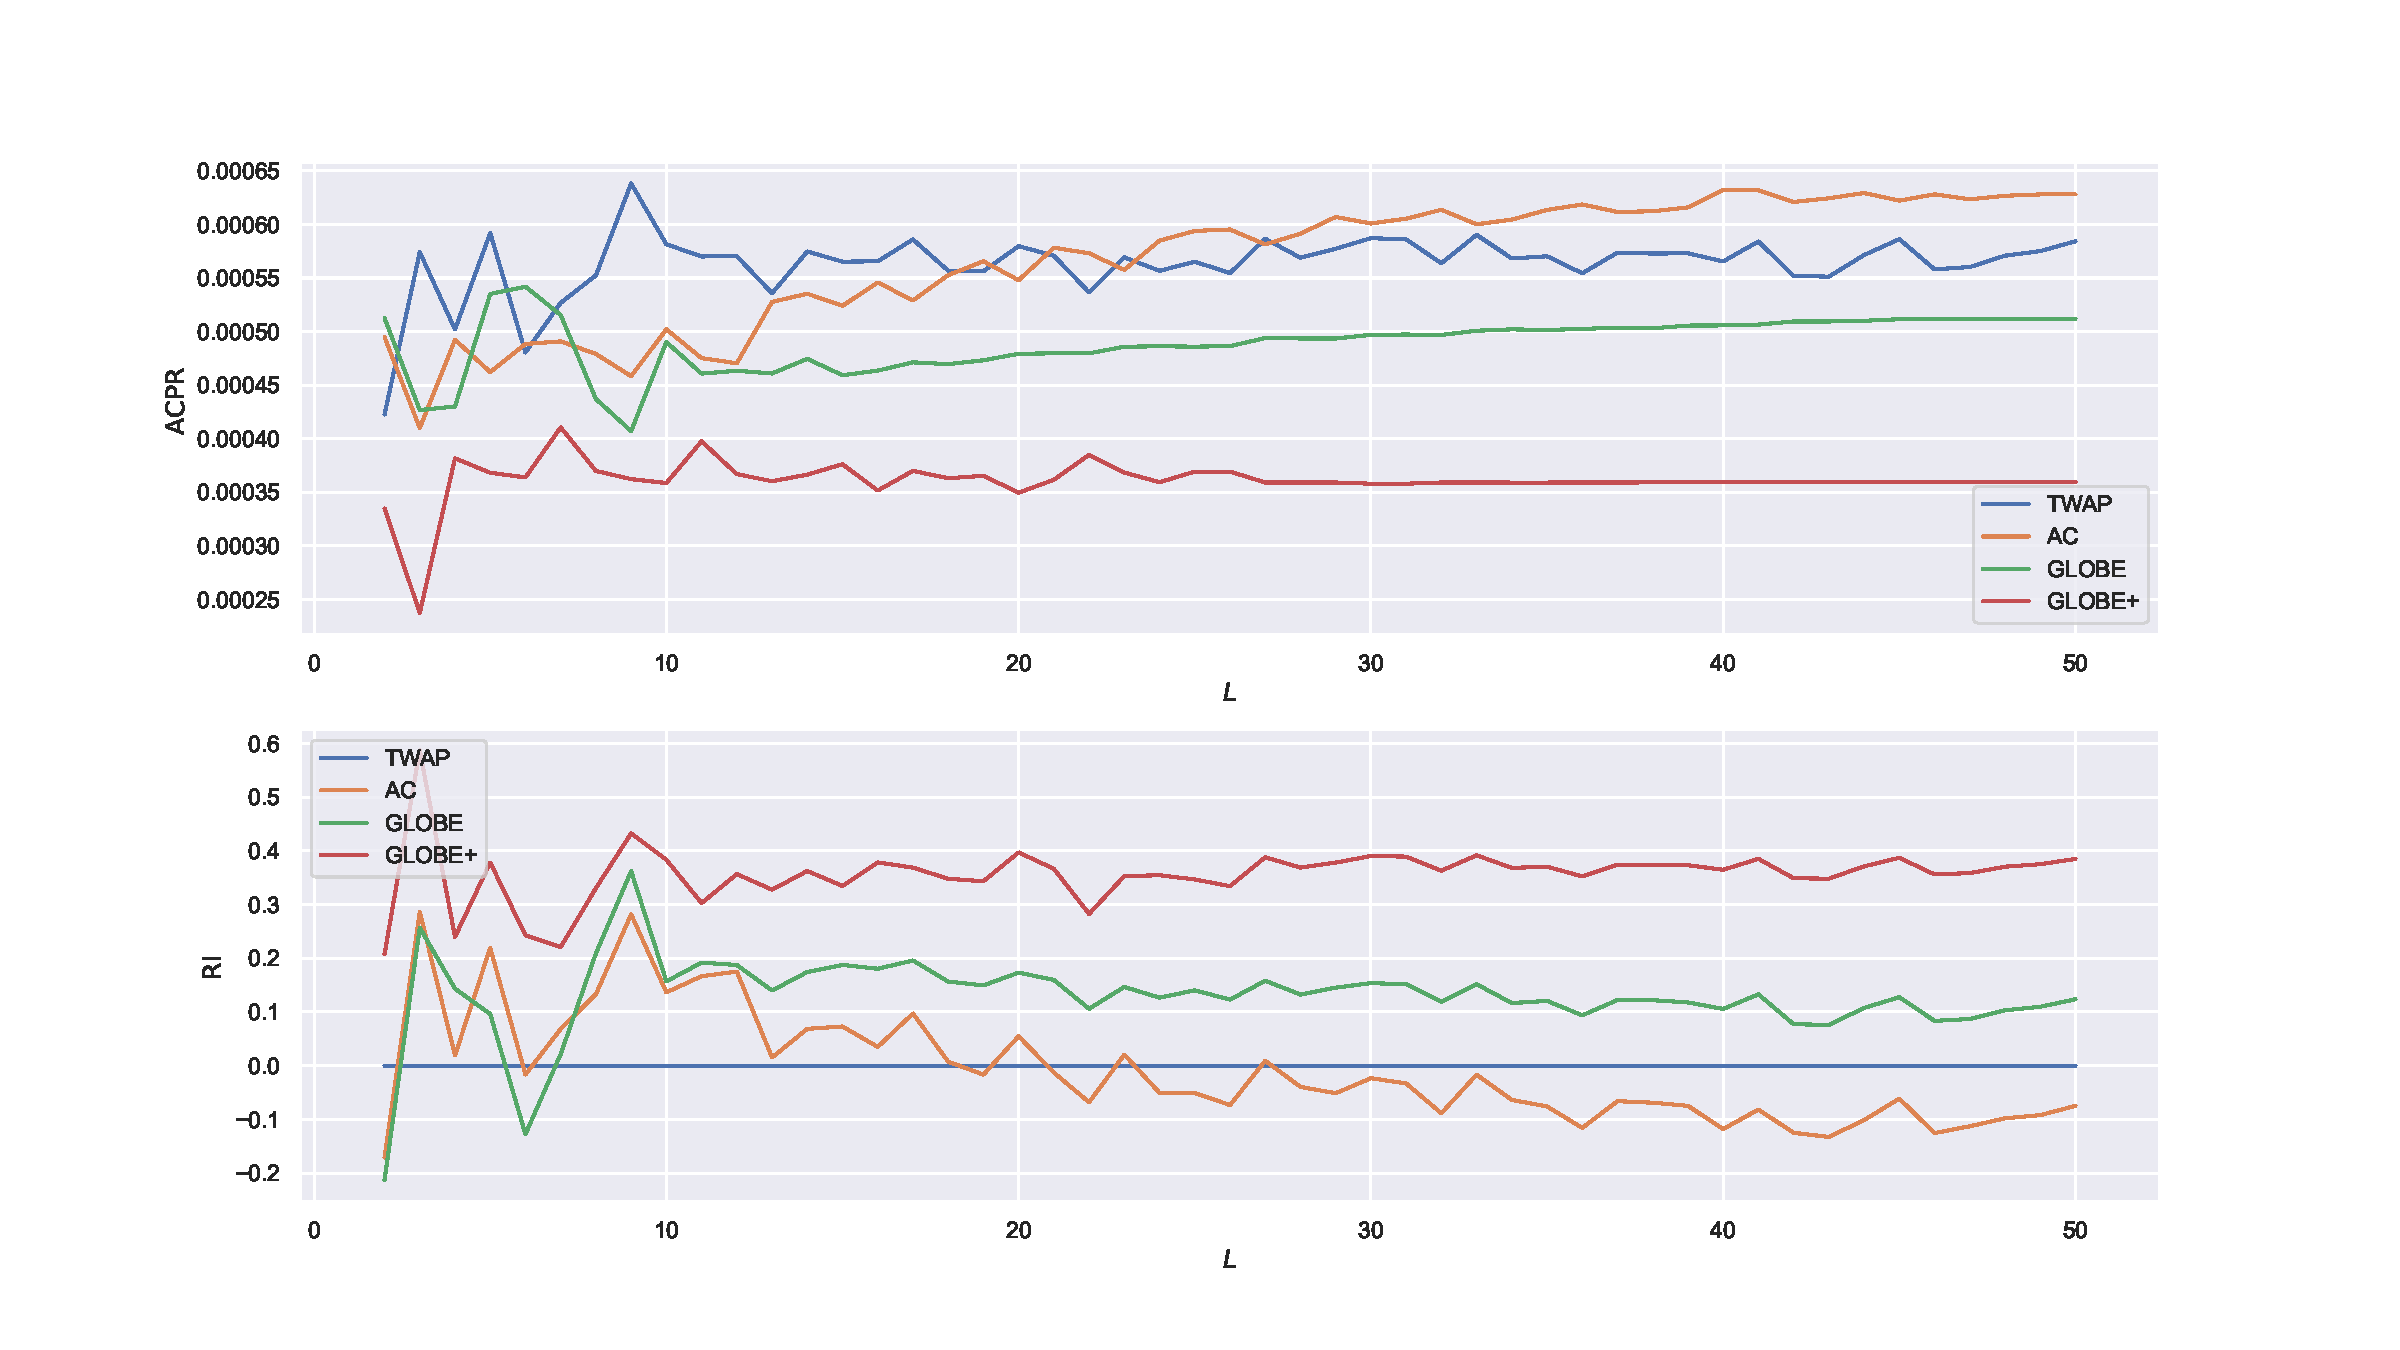
\includegraphics[width=0.83\linewidth]{USD_CNH_T+1 2022-10-04 T = 50 W = 500 x1000}
                \caption{USD\_CNH\_TOM 2022-10-04. $T = 50, W = 50\_000$}
            \end{figure}
            
        \end{frame}


        \begin{frame}{Пару слов о графиках}
            \begin{itemize}
                \item Было замечено, что алгоритмы довольно чуствительны к выбору параметров, однако, как их оценивать, авторам пока не очевидно...

                \item Более того стоит отметить, что более сложные алгоритмы чаще оказывались лучше при малых объемах. 
    
                \item При больших объемах ситуация неоднозначна. Возможно, параметры моделей зависят от объема. 
            \end{itemize}
        \end{frame}

    \section{Заключение}

        \begin{frame}{Подведение итогов}
            \begin{itemize}
                \item Была проведена работа по изучению абсолютно новой (для авторов) темы. 
                \item Остальная часть работы носила чисто прикладной характер.
                \item Реализовано и протестировано на реальных данных 3.5 алгоритма (TWAP, AC, GLOBE, GLOBE+). Эмпирически получено, что более сложные алгоритмы в среднем дают небольшой выигрыш.             
            \end{itemize}
        \end{frame}

        \begin{frame}{Что дальше?}
            \begin{itemize}
                \item Придумать и реализовать алгоритмы калибровки параметров для AC и GLOBE.
                \item Реализвоать и протестировать другие RL алгоритмы (например, основаные на Q-обучении).
                \item Возможно, попробовать наиболее удачные алгоритмы на реальном рынке. 
                \item Придумать, как можно улучшить данные алгоритмы. Возможно, придумать собственный.
            \end{itemize}
        \end{frame}

        \begin{frame}{Послесловие}
            \begin{figure}  
                \centering
                
\includegraphics[width=0.83\linewidth]{workflow.jpeg}
            \end{figure}
        \end{frame}

        \begin{frame}{Дисклеймер}
            \centering

            \bf\Large{Все лица и события вымышлены, совпадения случайны. В результате постановки никто из алгоритмов не пострадал.}
        \end{frame}
    \end{document}